%-------------------------------
%	PACKAGES AND OTHER DOCUMENT CONFIGURATIONS
%-------------------------------

% The \vref command specifies the location of the reference

\documentclass[
10pt, % Main document font size
a4paper, % Paper type, use 'letterpaper' for US Letter paper
oneside, % One page layout (no page indentation)
%twoside, % Two page layout (page indentation for binding and different headers)
headinclude,footinclude, % Extra spacing for the header and footer
BCOR5mm, % Binding correction
]{scrartcl}

% Roman numerals for sections and subsections
\renewcommand{\thesection}{\Roman{section}} 
%\renewcommand{\thesubsection}{\thesection.\Roman{subsection}}


%--------------------------------------------------------------
%	REQUIRED PACKAGES
%--------------------------------------------------------------

\usepackage[
nochapters, % Turn off chapters since this is an article        
beramono, % Use the Bera Mono font for monospaced text (\texttt)
%eulermath,% Use the Euler font for mathematics
pdfspacing, % Makes use of pdftex’ letter spacing capabilities via the microtype package
dottedtoc % Dotted lines leading to the page numbers in the table of contents
]{classicthesis} % The layout is based on the Classic Thesis style



\usepackage{arsclassica} % Modifies the Classic Thesis package

\usepackage[T1]{fontenc} % Use 8-bit encoding that has 256 glyphs

\usepackage[utf8]{inputenc} % Required for including letters with accents

\usepackage{libertinus} % The Libertinus font
%\usepackage[adobe-utopia]{mathdesign} % The Utopia font

%\usepackage[czech]{babel} % Český jazyk
\usepackage[english]{babel} % English

\usepackage{graphicx} % Required for including images
\graphicspath{{Figures/}} % Set the default folder for images

\usepackage{enumitem} % Required for manipulating the whitespace between and within lists

\usepackage{lipsum} % Used for inserting dummy 'Lorem ipsum' text into the template

\usepackage{subfig} % Required for creating figures with multiple parts (subfigures)

\usepackage{amsmath,amssymb,amsthm,amsfonts} % For including math equations, theorems, symbols, etc

\usepackage{varioref} % More descriptive referencing

\usepackage{geometry}

\usepackage{csquotes}


%------------------------------------------------------------
%	THEOREM STYLES
%------------------------------------------------------------

\theoremstyle{definition} % Define theorem styles here based on the definition style (used for definitions and examples)
\newtheorem{definition}{Definition}

\theoremstyle{plain} % Define theorem styles here based on the plain style (used for theorems, lemmas, propositions)
\newtheorem{theorem}{Theorem}
\newtheorem{preposition}{Preposition}
\newtheorem{corollary}{Corollary}

\theoremstyle{remark} % Define theorem styles here based on the remark style (used for remarks and notes)
\newtheorem{remark}{Remark}
\newtheorem{example}{Example}


%-------------------------------------------------------------
%	HYPERLINKS
%-------------------------------------------------------------

\hypersetup{
%draft, % Uncomment to remove all links (useful for printing in black and white)
colorlinks=true, breaklinks=true, bookmarks=true,bookmarksnumbered,
urlcolor=webbrown, linkcolor=RoyalBlue, citecolor=webgreen, % Link colors
pdftitle={}, % PDF title
pdfauthor={\textcopyright}, % PDF Author
pdfsubject={}, % PDF Subject
pdfkeywords={}, % PDF Keywords
pdfcreator={pdfLaTeX}, % PDF Creator
pdfproducer={LaTeX with hyperref and ClassicThesis} % PDF producer
}

 % Include the structure.tex file which specified the document structure and layout

%----------------------------------------------------
%	MATHEMATICS
%----------------------------------------------------

% Tělesa, obory íntegrity a metrické prostory
\newcommand{\C}{\mathbb{C}}
\newcommand{\R}{\mathbb{R}}
\newcommand{\N}{\mathbb{N}}
\newcommand{\Q}{\mathbb{Q}}
\newcommand{\Z}{\mathbb{Z}}
\renewcommand{\H}{\mathcal{H}} % Hilbert space
\renewcommand{\L}[2]{L^{#1}(#2)} % Lebesgueovy prostory

\newcommand{\vc}[1]{\boldsymbol{#1}} % vektor
\newcommand{\mat}[1]{\mathbf{#1}} % matice
\renewcommand{\i}{\mathrm{i}} % imaginární jednotka
\newcommand{\e}{\mathrm{e}} % Eulerovo číslo


\newcommand{\norm}[1]{\left \Vert #1 \right \Vert} % norma vektoru
\newcommand{\set}[1]{ \left \lbrace #1 \right \rbrace} % množina
\newcommand{\const}{\mathrm{konst}} % konstanta

\newcommand{\F}{\mathcal{F} } % Fourierova transformace
\newcommand{\La}{\mathcal{L}} % Laplaceova transformace

% Označení funkcí
\newcommand{\Res}[2]{\mathrm{Res}_{#1} \, #2 \,} % residuum
\newcommand{\sgn}{\, \mathrm{sign} \,} % signum
\newcommand{\tg}{\,\mathrm{tg}\,} % možné značení tangens


%Značení derivací a integrálů
\newcommand{\der}[2]{\frac{\mathrm{d}#1}{\mathrm{d}#2}} % obyčejná derivace
\newcommand{\pder}[2]{\frac{\partial #1}{\partial #2}} % parciální derivace
\newcommand{\tder}[3]{\left( \pder{#1}{#2} \right)_{#3 = \const}} % termodynamická derivace
\newcommand{\D}{\mathrm{d} } % integrační znamení
\newcommand{\DD}{\mathrm{D}} % absolutní derivace
\newcommand{\intR}{\int_{-\infty}^{\infty}} % integrál přes reálnou osu



% Značení posloupností, limit a sum
\newcommand{\sequence}[2]{ \left \lbrace #1 \right \rbrace_{#2=1}^\infty} % posloupnost
\newcommand{\sumnorm}[1]{\sum_{#1}^\infty} 
\newcommand{\limplus}[1]{\lim_{#1 \rightarrow + \infty}}
\newcommand{\limminus}[1]{\lim_{#1 \rightarrow - \infty}}
\newcommand{\cu}{\overset{u}\rightarrow} % uniform convergence
\newcommand{\cs}{\overset{s}\rightarrow} % strong convergence
\newcommand{\cw}{\overset{w}\rightarrow} % weak operator convergence
\newcommand{\slim}{\mathrm{s-}\lim} % strong limit
\newcommand{\ulim}{\mathrm{u-}\lim} % uniform limit

% Značení distribucí
\newcommand{\dual}[2]{\left \langle #1 ,#2 \right \rangle} % dualita
\newcommand{\tf}[1]{\mathcal{D}(#1)} % prostor testovacích funkcí
\newcommand{\dis}[1]{\mathcal{D'}(#1)} % prostor distribucí
\newcommand{\Schwartz}[1]{\mathcal{S}(#1)} % Schwartzův prostor
\newcommand{\weakstar}{\rightharpoonup^*} % slabá* konvergence 
\newcommand{\supp}{\mathrm{supp}\,} % nosič funkcí


% Značení operátorů
\newcommand{\op}[1]{\mathsf{#1}} %označení operátorů
\renewcommand{\o}[1]{\overline{#1}} %zjednodušení značení overline, často potřeba
\newcommand{\Ran}{\mathrm{Ran}\,}
\newcommand{\Ker}{\mathrm{Ker}\,}

% Označení spekter a měr

\newcommand{\mupp}{\mu_{\mathrm{pp}}}
\newcommand{\muac}{\mu_{\mathrm{ac}}}
\newcommand{\musing}{\mu_{\mathrm{sing}}}

\newcommand{\Hpp}{\H_{\mathrm{pp}}}
\newcommand{\Hac}{\H_{\mathrm{ac}}}
\newcommand{\Hsing}{\H_{\mathrm{sing}}}

\newcommand{\phimap}{\boldsymbol{\phi}}

\newcommand{\Lin}[1]{\mathcal L(#1)} % Include the mathematics.tex file which uses some mathematical operators

\hyphenation{Fortran hy-phen-ation} % Specify custom hyphenation points in words with dashes where you would like hyphenation to occur, or alternatively, don't put any dashes in a word to stop hyphenation altogether

%-------------------------------
%	TITLE AND AUTHOR(S)
%-------------------------------

\title{\normalfont\spacedallcaps{Methods of Modern Mathematical Physics}} % The article title

%\subtitle{Subtitle} % Uncomment to display a subtitle

\author{\spacedlowsmallcaps{Authors: Michael Reed, Barry Simon}} % The article author(s) - author affiliations need to be specified in the AUTHOR AFFILIATIONS block

\date{} % An optional date to appear under the author(s)




%-------------------------------------
%	TESTING
%-------------------------------------
% Load packages for testing
\usepackage{blindtext}
%\usepackage{showframe} % Uncomment to show boxes around the text area, margin, header and footer
\usepackage[inline]{showlabels}  \showlabels[\small\color{JungleGreen}]{}  % Uncomment to output the content of \label commands to the document where they are used


\begin{document}

%-------------------------------------------
%	HEADERS
%-------------------------------------------

\renewcommand{\sectionmark}[1]{\markright{\spacedlowsmallcaps{#1}}} % The header for all pages (oneside) or for even pages (twoside)
%\renewcommand{\subsectionmark}[1]{\markright{\thesubsection~#1}} % Uncomment when using the twoside option - this modifies the header on odd pages
\lehead{\mbox{\llap{\small\thepage\kern1em\color{halfgray} \vline}\color{halfgray}\hspace{0.5em}\rightmark\hfil}} % The header style

\pagestyle{scrheadings} % Enable the headers specified in this block





%-----------------------------------------
%	TABLE OF CONTENTS & LISTS OF FIGURES AND TABLES
%-----------------------------------------

\maketitle % Print the title/author/date block

\setcounter{tocdepth}{2} % Set the depth of the table of contents to show sections and subsections only

%\tableofcontents % Print the table of contents

%\listoffigures % Print the list of figures

%\listoftables % Print the list of tables






%--------------------------------------
%	ABSTRACT
%--------------------------------------

%\section*{Abstract} % This section will not appear in the table of contents due to the star (\section*)


%---------------------------------------
%	AUTHOR AFFILIATIONS
%---------------------------------------

\let\thefootnote\relax\footnotetext{* \textbf{Transcript:} Miroslav Burýšek, \textbf{Contact:} \href{miroslav@burysek.eu}{miroslav@burysek.eu} }

%--------------------------------------

%\newpage % Start the article content on the second page, remove this if you have a longer abstract that goes onto the second page

\setcounter{section}{5}
\section{Bounded Operators}

\subsection{Topologies on bounded operators}

one Banach space to another. In this chapter we will study $\Lin{X,Y}$ more
closely. We emphasize the case which will arise most frequently later, namely,
$\Lin{\H, \H} \equiv \Lin{H}$ where $\H$ is a separable Hilbert space. Theorem III.2
shows that $\Lin{X,Y}$ is a Banach space with the norm \begin{align}
    \norm{\op T} = \sup_{x \neq 0} \frac{\norm{\op T x}_Y}{\norm{x}_X} \:.
\end{align}
The induced topology on $\Lin{X,Y}$ is called the \textbf{uniform operator topology} (or \textbf{norm topology}). In this topology the map $[A,B] \mapsto BA$ of $\Lin{X,Y} \times \Lin{X,Y} \to \Lin{X,Z}$ is jointly continuous.
We now introduce two new topologies on $\Lin{X,Y}$, the weak and strong operator topologies. There are other interesting and useful topologies on $\Lin{X,Y}$, but we delay their introduction until we need them in a later volume (see however the discussion at the end of Section 6 and the Notes).

The \textbf{strong operator topology} is the weakest topology on $\Lin{X,Y}$ such that the maps \begin{align}
    E_x : \Lin{X,Y} \to Y 
\end{align}
given by $E_X(\op T) = \op T x$ are continuous for all $x \in X$. A neighborhood basis at the origin is given by sets of the form \begin{align}
    \set{\op S | \op S \in \Lin{X,Y} \:, \: \norm{\op S x_i}_Y < \varepsilon \:, \: i = 1, \cdots, n}
\end{align}
where $\set{x_i}_{i=1}^n$ is a finite collection of elements of $X$ and $\varepsilon$ is positive. In this topology a net $\set{T_\alpha}$ of operators converges to an operator $\op T$ (written $\op T_\alpha \cs \op T$ if and only if $\norm{\op T_\alpha x - \op T x}$ for all $x \in X$. The map $[\op A, \op B] \mapsto \op A \op B$ is separately but not jointly continuous if $X$, $Y$, and $Z$ are infinite dimensional (see Problem 6a, b). We sometimes denote strong limits by the symbol $\slim$.

The \textbf{weak operator topology} on $\Lin{X,Y}$ is the weakest topology such that the maps
\begin{align}
    E_{x, \ell} : \Lin{X,Y} \to \C 
\end{align}
given by $E_{x, \ell}(\op T) = \ell(\op T x)$ are all continuous for all $x \in X$, $\ell \in Y^\star$. A basis at the origin is given by sets of the form \begin{align}
    \set{\op S | \op S \in \Lin{X,Y} \:; \: |\ell_i(\op T x_j)| < \varepsilon \:; \: i = 1, \cdots , n \:; \: j = 1, \cdots, m} 
\end{align}
where $\set{x_i}_{i=1}^n$ and $\set{\ell_j}_{j=1}^m$ are finite families of elements of $X$ and $Y^\star$ respectively. A net of operators $\set{\op T_\alpha}$ converges to an operator $\op T$ in the weak operator topology (written $\op T_\alpha \cw \op T$) if and only if $|\ell (\op T_\alpha x) - \ell (\op T x)| \rightarrow 0$ for each $l \in Y^\star$ and $x \in X$. Notice that in the case $\Lin{\H}$, $T_\gamma \cw$ just means that the \enquote{matrix elements} $(y, \op T_\gamma x)$ converge to $(y, \op T x)$. In the weak topology the map $[\op A, \op B] \mapsto \op A \op B$ is separately, but not jointly continuous if $X$, $Y$ and $Z$ are infinite dimensional (see Problem 6c).

\begin{remark}
    The reader should not confuse the weak operator topology on $\Lin{X,Y}$ with the weak (Banach space) topology on $\Lin{X,Y}$. The former is the weakest topology such that the bounded linear functionals on $\Lin{X,Y}$ of the form $\ell(\cdot x)$ are continuous for all $x \in X$ and $\ell \in Y^\star$. The latter is the weakest topology such that \textit{all} bounded linear functionals on $\Lin{X,Y}$ are continuous (see Section VI.6).
\end{remark}

Notice that the weak operator topology is weaker than the strong operator topology which is weaker than the uniform operator topology. In general, the weak and strong operator topologies on $\Lin{X,Y}$ will not be first countable so that questions of compactness, net convergence, and sequential convergence are complicated. The following simple example illustrates the different topologies on $\Lin{\ell_2}$.

\begin{example}
    Consider the bounded operators on $\ell_2$.
    \begin{enumerate}
        \item Let $\op T_n$ be defined by \begin{align}
            \op T_n (\xi_1, \xi_2, \cdots) = \left( \frac{1}{n} \xi_1, \frac{1}{n} \xi_2, \cdots \right) \:.
        \end{align}
        Then $\op T_n \rightarrow 0$ uniformly.

        \item Let $\op S_n$ be defined by \begin{align}
            \op S_n(\xi_1, \xi_2, \cdots) = \left( 0,0, \cdots, 0, \xi_{n+1}, \xi_{n+2}, \cdots \right) \:.
        \end{align}
        Then $\op S_n \rightarrow 0$ strongly but not uniformly.

        \item Let $\op W_n$ be defined by \begin{align}
            \op W_n(\xi_1, \xi_2, \cdots) = \left( 0,0, \cdots, 0, \xi_1, \xi_2, \cdots \right) \:.
        \end{align}
        Then $\op W_n \rightarrow 0$ in the weak operator topology but not in the strong or uniform topologies.
    \end{enumerate}

\end{example}

The following result in the Hilbert space case is sometimes useful and provides
a nice application of the uniform boundedness theorem.

\begin{theorem}
    Let $\Lin{H}$ denote the bounded operators on a Hilbert space $\H$. Let $\op T_n$ be a \textit{sequence} of bounded operators and suppose that $(\op T_n x, y)$ converges as $n \rightarrow \infty$ for each $x,y \in \H$. Then there exists $\op T \in \Lin{\H}$ such that $\op T_n \cw \op T$.
\end{theorem}

\begin{proof}
    We begin by showing that for each $x$, $\sup_n \norm{\op T_n x} < \infty$. Since for any $x \in \H$, $(x, \op T_n y)$ converges we have \begin{align}
        \sup_n |(\op T_n x, y)| < \infty \:.
    \end{align}
    For each $n$, $\op T_n x \in \Lin{\H, \C}$, and since $\sup_n |(\op T_n x)(y)|_{\C} < \infty$, the uniform boundedness theorem implies that the operator norms of the $\op T_nx$ in $\Lin{\H, \C}$ is the same as its norm in $\H$; thus $\norm{\op T_n x}_{\H}$ is uniformly bounded.

    Now, we use the uniform boundedness theorem again. Since \begin{align}
        \sup_n \norm{\op T_n x}_{\H} < \infty \:,
    \end{align}
    we conclude \begin{align}
        \sup_n \norm{\op T_n}_{\Lin{\H}} < \infty \:.
    \end{align}
    Define $B(x,y) = \lim_n (\op T_n x, y)$. Then it is easily verified that $B(x,y)$ is sesquilinear and \begin{align}
        |B(x,y)| \leq \lim_n |(\op T_n x,y)| \leq \norm{x} \norm{y} (\sup_n \norm{\op T_n}) \:.
    \end{align}
    Thus $B(x,y)$ is a bounded sesquilinear form on $\H$ and so, by the corollary to the Riesz lemma, there is a bounded operator $\op T \in \Lin{\H}$ sush that $B(x,y) = (\op T x,y)$. Clearly $\op T_n \cw \op T$.
\end{proof}

If a sequence of operators $\op T_n$, on a Hilbert space has the property that $\op T_n x$ converges for each $x \in \H$, then there exists $\op T \in \Lin{\H}$ such that $\op T_n \cs \op T$. The reader is asked to prove this theorem and various generalizations in Problem 3.

Let $\op T \in \Lin{X,Y}$. The set of vectors $x \in X$ so that $\op T x = 0$ is called the \textbf{kernel} of $\op T$, written $\Ker \op T$. The set of vectors $y \in Y$ that $y = \op T x$ for some $x \in X$ is called the \textbf{range} of $\op T$, written $ \Ran \op T$. Notice that both $\Ker \op T$ and $\Ran \op T$ are subspaces. Ker $\op T$ is necessarily closed, but $\Ran \op T$ may not be closed (Problem 7).

\subsection{Adjoints}

In this section we define adjoints of bounded operators on Banach and Hilbert spaces. The reader should be cautioned at the outset that the Hilbert space adjoint of an operator $\op T \in \Lin{H}$ is not equal to the Banach space adjoint although it is closely related to it.

\begin{definition}
    Let $X$ and $Y$ be Banach spaces, $\op T$ a bounded linear operator from $X$ to $Y$. The Banach space \textbf{adjoint} of $\op T$, denoted by $\op T'$, is the bounded linear operator from $Y^\star$ to $X^\star$ defined by
    \begin{align}
        (\op T' \ell)(x) = \ell(\op T x) \quad \text{ for all } \quad \ell \in Y^\star \:, \: x \in X \:.
    \end{align}
\end{definition}

\begin{example}
    Let $X = \ell_1 = Y$ and let $\op T$ be the right shift operator
    \begin{align}
        \op T (\xi_1, \xi_2, \cdots) = (0, \xi_1, \xi_2, \cdots) \:.
    \end{align}
    Then $\op T' : \ell_\infty \to \ell_\infty$ is the operator
    \begin{align}
        \op T'(\xi_1, \xi_2, \cdots) = (\xi_2, \xi_3, \cdots) \:.
    \end{align}
    In this example, $\norm{\op T} = 1 = \norm{\op T'}$. In fact the norms of $\op T$ and $\op T'$ are always equal:
\end{example}

\begin{theorem}
    Let $X$ and $Y$ be Banach spaces. The map $\op T \mapsto \op T'$ is an isometric isomorphism of $\Lin{X,Y}$ into $\Lin{X^\star,Y^\star}$.
\end{theorem}

\begin{proof}
    The map $\op T \mapsto \op T'$ is linear. The fact that $\op T'$ is bounded and that the map is an isometry follows from the computation ($\ell \in Y^\star$)
    \begin{align}
        \norm{\op T}_{\Lin{X,Y}} = \sup_{\norm{x} \leq 1} \norm{\op T x}_Y
        = \sup_{\norm{\ell} \leq 1} \left( \sup_{\norm{x} \leq 1} |\ell(\op T x)|\right)
        = \sup_{\norm{\ell} \leq 1} \norm{\op T' \ell} = \norm{\op T'}_{\Lin{Y^\star, X^\star}} \:.
    \end{align}
    The second equality uses a corollary of the Hahn Banach theorem.
\end{proof}

We are mostly interested in the case where $\op T$ is a bounded linear transformation of a Hilbert space $\H$ to itself. The Banach space adjoint of $\op T$ is then a mapping of $\H^\star$ to $\H^\star$. Let $\op C : \H \to \H^\star$ be the map which assigns to each $y \in \H$, the bounded linear functional $(y, \cdot)$ in $\H^\star$. $\op C$ is a \textit{conjugate} linear isometry which is surjective by the Riesz lemma. Now define a map $\op T^\star : \H \to \H$ by \begin{align}
    \op T^\star = \op C^{-1} \op T' \op C \:.
\end{align}
Then $\op T^\star$ satisfies \begin{align}
    (x, \op T y) = (\op C x)(\op T y)= (\op T' \op C x)(y) = (\op C^{-1} \op T' \op C x, y) = (\op T^\star x,y) \:.
\end{align}

\begin{theorem}
    \begin{enumerate}
        \item $\op T \mapsto \op T^\star$ is a conjugate linear isometric isomorphism of $\Lin{\H}$ onto $\Lin{\H}$.
        \item $(\op T \op S)^\star = \op S^\star \op T^\star$.
        \item $(\op T^\star)^\star = \op T$.
        \item If $\op T$ has a bounded inverse, $\op T^{-1}$, then $\op T^\star$ has a bounded inverse and $(\op T^\star)^{-1} = (\op T^{-1})^\star$.
        \item The map $\op T \mapsto \op T^\star$ is always continuous in the weak and uniform operator topologies but is only continuous in the strong operator topology if $\H$ is finite dimensional.
        \item $\norm{\op T^\star \op T} = \norm{\op T}^2$.
    \end{enumerate}
\end{theorem}

\begin{proof}
    (1) follows from Theorem VI.2 and the fact that $\op C$ is an isometry. (2) and (3) are easily checked. Since $\op T^{-1} \op T = \op I = \op T \op T^{-1}$, we have from (2)
    \begin{align}
        \op T^\star (\op T^{-1})^\star = \op I^\star = \op I = \op I^\star = (\op T^{-1})^\star \op T^\star
    \end{align}
    which proves (4).
    TODO (5)
\end{proof}

\begin{definition}
    A bounded operator $\op T$ on a Hilbert space is called \textbf{self-adjoint} if $\op T = \op T^\star$.
\end{definition}

Self-adjoint operators play a major role in functional analysis and mathematical physics and much of our time is devoted to studying them. Chapter VII is devoted to proving a structure theorem for bounded self-adjoint operators. In Chapter VIII we introduce unbounded self-adjoint operators and continue their study in Chapter X. We remind the reader that on $\C^n$, a linear transformation is self-adjoint if and only if its matrix in any orthonormal basis is invariant under the operation of reflection across the diagonal followed by complex conjugation.

An important class of operators on Hilbert spaces is that of the projections.

\begin{definition}
    If $\op P \in \Lin{\H}$ and $\op P^2 = \op P$, then $\op P$ is called a \textbf{projection}. If in addition $\op P = \op P^\star$, then $\op P$ is called an \textbf{orthogonal projection}.
\end{definition}

Notice that the range of a projection is always a closed subspace on which $\op P$ acts like the identity. If in addition $\op P$ is orthogonal, then $\op P$ acts like the zero operator on $(\Ran \op P)^\bot$. If $x = y + z$, with $y \in \Ran \op P$ and $z \in (\Ran \op P)^\bot$, is the decomposition guaranteed by the projection theorem, then $\op P x =y$. $\op P$ is called the orthogonal projection onto $\Ran \op P$. Thus, the projection theorem sets up a one to one correspondence between orthogonal projections and closed subspaces. Since orthogonal projections arise more frequently than nonorthogonal ones, we normally use the word projection to mean orthogonal projection.

\subsection{The spectrum}

If $\op T$ is a linear transformation on $\C^n$, then the eigenvalues of $\op T$ are the complex numbers $\lambda$ 
such that the determinant of $( \lambda \op J - \op T )$ is equal to zero. 
The set of such $\lambda$ is called the spectrum of $\op T$. It can consist of at most $n$ points since $\det (\lambda \op I - \op T)$ is a polynomial of degree $n$. If $\lambda$ is not an eigenvalue, then $\lambda \op I - \op T$ has an inverse since $\det (\lambda \op I - \op T) \neq 0$.
The spectral theory of operators on infinite-dimensional spaces is more complicated, more interesting, and very important for an understanding of the operators themselves.

\begin{definition}
    Let $\op T \in \Lin{X}$. A complex number $\lambda$ is said to be in the \textbf{resolvent set} $\rho(\op T)$ of $\op T$ if $\lambda \op I - \op T$ is a bijection with a bounded inverse. $\op R_{\lambda}(\op T) = (\lambda \op I - \op T)^{-1}$ is called the \textbf{resolvent} of $\op T$ at $\lambda$. If $\lambda \neq \rho(\op T)$, then $\lambda$ is said to be in the \textbf{spectrum} $\sigma(\op T)$ of $\op T$.
\end{definition}

We note that by the inverse mapping theorem, $\lambda \op I - \op T$ automatically has a bounded inverse if it is bijective. We distinguish two subsets of the spectrum.

\begin{definition}
    Let $\op T \in \Lin{H}$.
    \begin{enumerate}
        \item An $x \neq 0$ which satisfies $\op T x = \lambda x$ for some $\lambda \in \C$ is called an \textbf{eigenvector} of $\op T$; $\lambda$ is called the corresponding \textbf{eigenvalue}. If $\lambda$ is an eigenvalue, then $\lambda \op I - \op T$ is not injective so $\lambda$ is in the spectrum of $\op T$. The set of all eigenvalues is called the \textbf{point spectrum} of $\op T$.
        \item If $\lambda$ is not an eigenvalue and if $\Ran (\lambda \op I - \op T)$ is not dense, then $\lambda$ is said to be in the \textbf{residual spectrum}.
    \end{enumerate}
\end{definition}

At the end of this section we present an example which illustrates these kinds of spectra. The reason that we single out the residual spectrum is that it does not occur for a large class of operators, for example, for self-adjoint operators (see Theorem VI.8).

The spectral analysis of operators is very important for mathematical physics. For example, in quantum mechanics the Hamiltonian is an unbounded self-adjoint operator on a Hilbert space. The point spectrum of the Hamil- tonian corresponds to the energy levels of bound states of the system. The rest of the spectrum plays an important role in the scattering theory of the system (see Chapter XII).

We will shortly prove that the resolvent set $\rho(\op T)$ is open and that $\op R_{\lambda}(\op T)$ is an analytic operator-valued function on $\rho(\op T)$. This fact allows one to use complex analysis to study $\op R_{\lambda}(\op T)$ and thus to obtain information about $\op T$. We begin
with a brief aside about vector-valued analytic functions.

Let $X$ be a Banach space and let $D$ be a region in the complex plane, i.e. a connected open subset of $\C$. A function, $x(\cdot)$, defined on $D$ with values in $X$, is said to be \textbf{strongly analytic} at $z_0 \in D$ if the limit of $\frac{x(z_0+h)-x(z_0)}{h}$ exists in $X$ as $h$ goes to zero in $\C$. Starting from this point one can develop a theory of vector-valued analytic functions which is almost exactly parallel to the usual theory; in particular, a strongly analytic function has a norm-convergent Taylor series. We do not repeat this development here; see the notes for references. We do want to discuss one important point. There is another natural way to define Banach-valued analytic functions. Namely: a
function $x(\cdot)$ on $D$ with values in $X$ is said to be \textbf{weakly analytic} if $\ell(x(\cdot))$ is a complex valued analytic function on $D$ for each $\ell \in X^\star$. Although this second definition of analytic is a priori weaker than the first, the two definitions are equivalent, a fact we will prove in a moment. This is very important, since weak analyticity is often much easier to check.

\begin{lemma}
    Let $X$ be a Banach space. Then a sequence $\set{x_n}$ is Cauchy if and only if $\set{\ell(x_n)}$ is Cauchy, uniformly for $\ell \in X^\star$, $\norm{\ell} \leq 1$.
\end{lemma}

\begin{proof}
    If $\set{x_n}$ is Cauchy, then $|\ell(x_n) - \ell(x_m)| \leq \norm{x_n-x_m}$ for all $\ell$ with $\norm{\ell} \leq 1$, so $\set{\ell(x_n)}$ is Cauchy uniformly. Conversely,
    \begin{align}
        \norm{x_n-x_m} = \sup_{\norm{\ell} \leq 1} |\ell(x_n-x_m)| \:.
    \end{align} 
    Thus, if $\set{\ell(x_n)}$ is Cauchy, uniformly for $\norm{\ell} \leq 1$, then $\set{x_n}$ is norm-Cauchy.
\end{proof}

\begin{theorem}
    Every weakly analytic function is strongly analytic.
\end{theorem}

\begin{proof}
    Let $x(\cdot)$ be a weakly analytic function on $D$ with values in $X$.Let $z_0 \in D$ and suppose $\Gamma$ is a circle in $D$ containing $z_0$ whose interior is contained in $D$. If $\ell \in X^\star$ then $\ell(x(z))$ is analytic and
    \begin{align}
        \ell \left( \frac{x(z_0+h)-x(z_0)}{h}\right) - \der{}{z} \ell(x(z_0)) = \\
        = \frac{1}{2 \pi \i} \oint_\Gamma \left[ \frac{1}{h} \left( \frac{1}{z-(z_0+h)} - \frac{1}{z-z_0} \right) - \frac{1}{(z-z_0)^2} \right] \ell (x(z)) \, \D z \:.
    \end{align}
    Since $\ell(x(z))$ is continuous on $\Gamma$ and $\Gamma$ is compact, $|\ell(x(z)) \leq C_\ell$ for all $z \in \Gamma$. Regarding $x(z)$ as a family of mappings $x(z) : X^\star \to \C$ we see that $x(z)$ is pointwise bounded at each $\ell$ so by the uniform boundedness theorem $\sup_{z \in \Gamma} \norm{x(z)} \leq C < \infty$. Thus \begin{align}
        \left| \ell \left( \frac{x(z_0+h)-x(z_0)}{h}\right) - \der{}{z} \ell(x(z_0)) \right| \leq \\
        \leq \frac{1}{2 \pi} \norm{\ell} \left( \sup_{z \in \Gamma} \norm{x(z)} \right) \oint_\Gamma \left| \frac{1}{(z-(z_0+h))(z-z_0)} - \frac{1}{(z-z_0)^2}\right| \, \D z
    \end{align}

\end{proof}
\section{Ergodic theory: An Introducion}

In this section we give a brief introduction to ergodic theory. For our discussion we need several concepts not formally defined until Chapter VI: adjoint operators, projection operators, and the kernel and range of an operator. Any reader not already familiar with these concepts should consult Chapter VI. We give this discussion here because ergodic theory illustrates nicely the power and limitations of Hilbert-space methods and serves as a nice example of the main theme of these books, namely the interplay between functional analysis and mathematical physics. We will see that it is useful to reformulate the question of why macroscopic systems approach equilibrium in terms of abstract spaces, but that one must pay a price: The natural question in the abstract setting is slightly different from the original question and one may be tempted to accept weaker results. The statement \enquote{any system approaches an equilibrium state} is sometimes known as the zeroth law of thermodynamics. From a microscopic point of view it is perhaps surprising that any system should approach equilibrium since microscopically there is no steady state and therefore no equilibrium.
Nevertheless, any attempt at a microscopic justification of thermodynamics must explain why the zeroth laws holds macroscopically. There is far from universal agreement among physicists as to what constitutes a justification of the zeroth law, but we would like to avoid a discussion of the pros and cons of the many different approaches which have been suggested (however, see the Notes). The approach that we use is generally accepted by most physicists. The first basic idea is that thermodynamical systems undergo fluctuations (see Problem 17); put differently, by their very nature the laws of thermodynamics are not absolute statements about a system at a fixed time but are statements about measurements made ver time periods long with respect to some characteristic times such as relaxation or collision times. Thus, thermodynamics deals with average measurements of observables over a time period $T$. Since the collision times, etc., are dependent on the dynamics, one can only hope to prove thermodynamic statements about the limit as $T \rightarrow \infty$.
How large $T$ has to be for the average over the interval $T$ to be approximately equal to the limit is a detailed dynamical question, but in specific cases one would hope to be able to prove something.
Let us suppose that we describe the state of a classical mechanical system
by a point in some phase space $\Gamma$. For each time $t$; there is a map $\op T_t : \Gamma \to \Gamma$, where $\op T_t x$ is the state which results by taking a state $x$ at $t_0$ and waiting until $t_0 + t$ (we are assuming time-translation invariance so $t_0$ never enters).
Obviously, $\op T_{t+s} = \op T_t \op T_s$. In classical mechanics, the observables of the system like energy or angular momentum are functions on phase discussion above suggests that we study
\begin{align}
    \lim_{T \rightarrow \infty} \frac{1}{T} \int_0^T f(\op T_t x) \, \D t \:.
\end{align}
We would like to show that the limit exists, at least for continuous functions. Typically $\Gamma$ is a metric space, so \enquote{continuous} has a meaning. Not only would we like the limit to exist, but it should be independent of the initial point $x$ or at least only dependent on a few \enquote*{macroscopic} observables we can associate with an equilibrium state. For systems which are time-translation independent, the energy is a conserved quantity, so the average-energy is the initial energy—thus we cannot hope for measurements to be independent of the initial energy. Therefore, for each energy $E$ we look at the constant energy surface, $\Omega_E$, in phase space, and for each  $w \in \Omega_E$ and each continuous function $f$ on $\Omega_E$ we hope that
\begin{align}
    \lim_{T \rightarrow \infty} \frac{1}{T} \int_0^T f(\op T_t w) \, \D t
\end{align}
exists and is a number, $\mu(f)$, independent of $w$. The map $f \mapsto \mu(f)$ clearly has three properties:
\begin{enumerate}
    \item $\mu(1)=1$.
    \item $\mu$ is linear.
    \item $\mu(f) \geq 0$ if $f \geq 0$.
\end{enumerate}
We will eventually see (Section I[V.4) that such a $\mu$ is always associated with a measure $\hat{mu}$ on $\Omega_E$ with $\hat{\mu}(\Omega_E) = 1$, so that
\begin{align}
    \mu(f) = \int_{\Omega_E} f(w) \, \D \hat{\mu}(w) \:.
\end{align}
From now on we denote linear functional $\mu$ and the measure $\hat{\mu}$, by the same letter $\mu$.

To summarize: We have shown that if
\begin{align}
    \lim_{T \rightarrow \infty} \frac{1}{T} \int_0^T f(\op T_t w) \, \D t
\end{align}
exists for each fixed $w$ and is independent of $w \in \Omega_E$, then there is a measure $\mu$ on $\Omega_E$ so that
\begin{align}
    \lim_{T \rightarrow \infty} \frac{1}{T} \int_0^T f(\op T_t w) \, \D t = \int_{\Omega_E} f(w) \, \D \mu(w) \:.
\end{align}
The measure $\mu$ has a very important property. Let $s$ be fixed and suppose $\chi_F$ is the characteristic function of a measurable set $F \subset \Omega_E$. The \begin{align}
    \frac{1}{T} \int_0^T \chi_{\op T_s^{-1} F} (\op T_t w) \, \D t = \frac{1}{T} \int_0^T \xi_F (\op T_s \op T_t w) \, \D t
\end{align}
so if the $\lim_{T \rightarrow \infty}$ exists, then $\mu(\op T_s^{-1}F) = \mu(F)$, that is, the measure is \textbf{invariant}. We also say that $\op T$ is \textbf{measure preserving}. Classical mechanical systems come equipped with a natural invariant measure: if $\Gamma = \R^{6N}$ ($N$ is the number of particles), the measure $\D^{3N} q \D^{3N} p$ is known to be invariant under the Hamiltonian flow (Liouville’s theorem). This measure has a restriction to $\Omega_E$ given formally by
\begin{align}
    \mu_E(F) = \int_F \delta \left[ H(p,q) - E \right] \, \D^{3N} p \D^{3N} q
\end{align}
where $H(p,q)$ is the Hamiltonian.
Explicitly, if we pick a set of local coordinates at $x \in \Omega_E$, say $Q_1, \cdots, Q_{6N-1}$, which are orthogonal and normalized, then
\begin{align}
    \D \mu_E = C \D^{6N-1} Q/ |\nabla H| \:,
\end{align}
$C$ is picked so that $\mu_E(\Omega_E) = 1$. Thus, the goal in justifying the zeroth law is to consider \begin{align}
    \op M_T(f)(w) = \frac{1}{T} \int_0^T f(\op T_t w) \, \D t
\end{align}
and to prove that in a suitable sense the function $(\op M_T f)(w)$ converges as $T \rightarrow \infty$ to the constant function with value
\begin{align}
    \int_{\Omega_E} f(w) \, \D \mu_E(w) \:.
\end{align}

Notice that if we can prove this, we will have proven much more; not only will we have shown that measurements over long periods of time are independent of the initial conditions (except for the energy), but we will have shown that the equilibrium state is described by a measure in phase space and this measure is
\begin{align}
    \int_F \delta \left[ H(p,q) - E \right] \, \D^{3N} p \D^{3N} q
\end{align}
the \enquote{microcanonical ensemble}.

\section{Domains, graphs, adjoints and spectrum}

It is a fact of life that many of the most important operators which occur in mathematical physics are not bounded. In this chapter we will introduce some of the basic definitions and theorems necessary for dealing with unbounded operators on Hilbert spaces. The Hellinger-Toeplitz theorem (see Section III.5) says that an everywhere-defined operator $\op A$ which satisfies $(\op A \phi, \psi) = (\phi, \op A \psi) $ is necessarily a bounded operator suggesting that a general unbounded operator $\op T$ will only be defined on a dense linear subset of the Hilbert space.
Thus an \textbf{operator} on a Hilbert space $\H$ is a linear map from its domain, a linear subspace of $\H$, into $\H$. Unless we specify otherwise, we will always suppose that the domain is dense. This subspace, which we denote by $D( \op T)$, is called the \textbf{domain} of the operator $\op T$. So, to identify an unbounded operator on a Hilbert space one must first give the domain on which it acts and then specify how it acts on that subspace.

\begin{example}[The position operator]
Let $\H = \L{2}{\R}$ and let $D(\op T)$ be the set of functions $\phi$ in $\L{2}{\R}$ which satisfy $\intR x^2 |\phi(x)|^2 \, \D x < \infty$. For $\phi \in D(\op T)$ define $(\op T \phi)(x) = x \phi(x)$. It is clear that $\op T$ is unbounded since if we choose $\phi$ to have support near plus or minus infinity, we can make $\norm{\op T \phi}$ as large as we like while keeping $\norm{\phi} =1$. Of course, even if $\phi \notin D(\op T)$, $x \phi(x)$ has a well- defined meaning as a function, but it is not in $\L{2}{\R}$. Thus, if we want to deal only with the Hilbert space $\L{2}{\R}$ we must restrict the domain of $\op T$. The domain we have chosen is the largest one for which the range is in $\L{2}{\R}$.
\end{example}

\begin{example}
Let $\H = \L{2}{\R}$ and $D(\op T)= \Schwartz{\R}$. On $D(\op T)$ define $\op T \psi = - \psi"(x) + x^2 \psi(x)$. If $\phi_n(x)$ is the $n$-th Hermite function (see the appendix to Section V.3), then $\phi_n \in D(\op T)$ and $\op T\phi_n(x) = (2n+1) \phi_n(x)$. Thus $\op T$ must be unbounded since it has arbitrarily large eigenvalues.
\end{example}

The notion of the graph of a linear transformation, introduced by von Neumann, is very useful for studying unbounded operators.

\begin{definition}
The \textbf{graph} of the linear transformation $\op T$ is the set of pairs
\begin{align}
    \set{[\phi, \op T \phi] | \phi \in D(\op T)} \:.
\end{align}
The graph of $\op T$, denoted by $\Gamma(\op T)$, is thus a subset of $\H \times \H$ which is a Hilbert space with inner product \begin{align}
    \left([\phi_1, \psi_1], [\phi_2, \psi_2] \right) = (\phi_1, \phi_2) + (\psi_1, \psi_2) \:.
\end{align}
$\op T$ is called a \textbf{closed} operator if $\Gamma(\op T)$ is a closed subset of $\H \times \H$.
\end{definition}

\begin{definition}
    Let $\op T_1$ and $\op T$ be operators on $\H$. If $\Gamma(\op T_1) \supset \Gamma(\op T)$, then $\op T_1$ is said to be an \textbf{extension }of $\op T$ and we write $\op T_1 \supset \op T$. Equivalently, $\op T_1 \supset \op T$ if and only if $D(\op T_1) \supset D(\op T)$ and $\op T_1 \phi = \op T \phi$ for all $\phi \in D(\op T)$.
\end{definition}

\begin{definition}
An operator $\op T$ is \textbf{closable} if it has a closed extension. Every closable operator has a smallest closed extension, called its \textbf{closure}, which we denote by $\o{\op T}$.   
\end{definition}


A natural way to try to obtain a closed extension of an operator $\op T$, is to take the closure of its graph in $\H \times \H$. The trouble with this is that $\Gamma(\op T)$ may not be the graph of an operator (for example, see Problem 1). However, most operators which we deal with will be symmetric operators (introduced Section VIII.2) and we will see that they always have closed extensions.

\begin{proposition}
If $\op T$ is closable, then $\Gamma(\o{\op T}) = \o{\Gamma(\op T)}$.
\end{proposition}

\begin{proof}
Suppose that $\op S$ is a closed extension of $\op T$. Then $\o{\Gamma(\op T)} \subset \Gamma(\op S)$ so if $[0, \psi] \in \o{\Gamma(\op T)}$ then $\psi = 0$.  

Define $\op R$ with $D(\op R) = \set{\psi | [\psi, \phi] \in \o{\Gamma(\op T)} \text{ for some } \phi}$ by $\op R \psi = \phi$ where $\phi \in \H$ is the unique vector so that $[\psi, \phi] \in \o{\Gamma(\op T)}$. Then
$\Gamma(\op R) = \o{\Gamma(\op T)}$ so $\op R$ is a closed extension of $\op T$. But $\op R \subset \op S$ which is an arbitrary
closed extension, so $\op R= \op T$.
\end{proof}

The following example illustrates the concepts we have just introduced.

\begin{example}
Let $\H = \L{2}{\R}$, $D(\op T) = C_0^\infty(\R)$ and $D(\op T_1) = C_0^1(\R)$, the once continuously differentiable functions with compact support.
Let $\op T f= \i f'(x)$ if $f \in D(\op T)$ and $\op T_1 f= \i f'(x)$ if  $f \in D(\op T_1)$. $\op T_1$ is an extension of $\op T$.

We will show that $\o{\Gamma(\op T)} \supset \Gamma(\op T_1)$. When we prove that $\op T$ is symmetric and therefore closable, it will follow that $\op T$ extends $\op T_1$. 

First we introduce the approximate identity, $\set{j_\varepsilon(x)}$. Let $j(x)$ be any positive, infinitely differentiable function with support in $(-1, 1)$ so that $\intR j(x) \D x = 1$. Define $j_\varepsilon(x) = \frac{1}{\varepsilon} j(\frac{x}{\varepsilon})$. If $\phi \in D(\op T_1)$, set \begin{align}
    \phi_\varepsilon(x) = \intR j_\varepsilon (x-t) \phi(t) \, \D t \:.
\end{align}
Then \begin{align}
    |\phi_\varepsilon(x) - \phi(x)| \leq \intR j_\varepsilon (x-t) |\phi(t) - \phi(x)| \, \D t\leq \\
    \leq \left( \sup_{t : |x-t| < \varepsilon} |\phi(t) - \phi(x)| \right) \intR j_\varepsilon (x-t) \, \D t=  \sup_{t : |x-t| < \varepsilon} |\phi(t) - \phi(x)| \:. \nonumber
\end{align}


Since $\phi$ has compact support, it is uniformly continuous which implies that $\phi_\varepsilon \rightarrow \phi$ uniformly. Since the $\phi_\varepsilon$ have support in a fixed compact set, $\phi_\varepsilon \rightarrow \phi$ in $\L{2}{\R}$.

Similarly,
\begin{align}
    \i \der{}{x} \phi_\varepsilon(x) 
    =&
    \intR \i \der{}{x} j_\varepsilon (x-t) \phi(t) \, \D t 
    = 
    \intR - \i \left( \der{}{t} j_\varepsilon (x-t) \right) \phi(t) \, \D t 
    = \\ =&
    \intR j_\varepsilon(x-t) \i \der{}{t} \phi(t) \, \D t 
    \overset{\L{2}{\R}} \longrightarrow
     \i  \der{}{x} \phi(x) \:. \nonumber
\end{align}

Since $j_\varepsilon(x)$ has compact support and is infinitely differentiable, $\phi_\varepsilon \in C_0^\infty(\R)$.
Thus, $\phi_\varepsilon \in D(\op T)$ for each $\varepsilon >0$. What we have shown above is that \begin{align}
    \phi_\varepsilon\overset{\L{2}{\R}} \longrightarrow \phi \:, 
	\quad     
    \op T \phi_\varepsilon \overset{\L{2}{\R}} \longrightarrow \op T \phi \:.
\end{align}
Thus, the closure of the graph of $\op T$ contains the graph of $\op T_1$. The notion of adjoint operator can be extended to the unbounded case.
\end{example}

\begin{definition}
Let $\op T$ be a densely defined linear operator on a Hilbert space $\H$. Let $D(\op T^\star)$ be the set of $\phi \in \H$ for which there is an $\eta \in \H$ with
\begin{align}
    (\op T \psi, \phi) = (\psi, \eta) \quad \text{for all } \psi \in D(\op T) \:. \label{eq:VIII.1}
\end{align}
For each such $\phi \in D(\op T^\star)$ we define $\op T^\star \phi = \eta$. $\op T^\star$ is called the \textbf{adjoint} of $\op T$. By the Riesz lemma, $\phi \in D(\op T^\star)$ if and only if $|(\op T \psi, \phi)| \leq C \norm{\psi}$ for all $\psi \in D(\op T)$.
\end{definition}


We note that $\op S \subset \op T$ implies $\op T^\star \subset \op S^\star$. Notice that for $\eta$ to be uniquely determined by \eqref{eq:VIII.1} we need the fact that $D(\op T)$ is dense. Unlike the case of bounded operators, the domain of $\op T^\star$ may not be dense as the following example shows. As a matter of fact it is possible to have $D(\op T^\star) = \set{0}$.

\begin{example}
Suppose that $f$ is a bounded measurable function, but that $f \notin \L{2}{\R}$. Let $D(\op T) = \set{\psi \in \L{2}{\R} | \intR f(x) \psi(x) \, \D x < \infty  }$. $D(\op T)$ certainly contains all the $L^2$ functions with compact support so $D(\op T)$ is dense in $\L{2}{\R}$. Let $\psi_0$ be some fixed vector in $\L{2}{\R}$ and define $\op T \psi = (f, \psi) \psi_0$ for $\psi \in D(\op T)$. Suppose that $\phi \in D(\op T^\star)$, then for all $\psi \in D(\op T)$
\begin{align}
    (\psi, \op T^\star \phi) = (\op T \psi, \phi) = ((f, \psi) \psi_0, \phi) = \o{(f, \psi)} (\psi_0, \phi) = (\psi, (\psi_0, \phi) f) \:. 
\end{align}
Thus $\op T^\star \phi = (\psi_0, \phi) f$. Since $f \notin \L{2}{\R}$, $(\psi_0, \phi) = 0$. Thus any $\phi \in D(\op T^\star)$ is orthogonal to $\psi_0$, so $D(\op T^\star)$ is not dense. In fact, $D(\op T^\star)$ is just the vectors perpendicular to $\psi_0$, and on that domain $\op T^\star$ is the zero operator.
\end{example}

If the domain of $\op T^\star$ is dense, then we can define $\op T^{\star \star} = (\op T^\star)^\star$. There is a simple relationship between the notions of adjoint and closure.

\begin{theorem}
Let $\op T$ be a densely defined operator on a Hilbert space $\H$. Then:
\begin{itemize}
    \item $\op T^\star$ is closed.
    \item $\op T$ is closable if and only if $D(\op T^\star)$ is dense in which case $\o{\op T} = \op T^{\star \star}$.
    \item If \,$\op T$ is closable, then $(\o{\op T})^\star = \op T^\star$.
\end{itemize}

\end{theorem}

\begin{proof}
We define a unitary operator $\op V$ on $\H \times \H$ by
\begin{align}
    \op V [\phi, \psi] = [-\psi, \phi] \:.
\end{align}
Since $\op V$ is unitary, $\op V[E^\bot] = (\op V[E])^\bot$ for any subspace $E$. Let $\op T$ be a linear operator on $\H$ and suppose $[\phi, \eta] \subset \H \times \H$. Then $[\phi, \eta] \in \op V[\Gamma(\op T)]^\bot$ if and only if $\left( [\phi, \eta], [- \op T \psi, \psi] \right) = 0$ for all $\psi \in D(\op T)$ which holds if and only if $(\phi, \op T \psi) = (\eta, \psi)$ for all $\psi \in D(\op T)$, that is, if and only if $[\phi, \eta] \in \Gamma(\op T^\star)$. Thus $\Gamma(\op T^\star) = \op V \left[\Gamma(\op T) \right]^\bot$. 
Since $\op V[\Gamma(\op T)]^\bot$ is always a closed subspace\footnote[1]{MB: If $M$ is an subspace of $\H$, then $M^\bot$ is always closed. If $\set{y_n}_n \subset M^\bot$ which $y_n \rightarrow y$, then $(y_n,x) = 0$ for all $x \in M$ and so $(y,x) = 0$ for all $x \in M$, therefore $y \in \H$. Also $(M^\bot)^\bot = \o{M}$.} of $\H \times \H$, this proves (1).

To prove (2), observe that $\Gamma(\op T)$ is a linear subset of $\H \times \H$ so
\begin{align}
    \o{\Gamma(\op T)} = \left[ \Gamma(\op T)^\bot \right]^\bot = \left[ \op V^2 \Gamma(\op T)^\bot \right]^\bot = \left[ \op V(\op V \Gamma(\op T))^\bot \right]^\bot \:.
\end{align}
By the proof of (1), $\op V [\Gamma (\op T)]^\bot = \Gamma (\op T^\star)$, and if $\op T^\star$ is densely defined, then 
\begin{align}
    \o{\Gamma(\op T)} = \left[ \op V(\op V \Gamma(\op T))^\bot \right]^\bot = \left[ \op V(\Gamma(\op T^\star))\right]^\bot = \Gamma(\op T^{\star \star}) \:, 
\end{align}
so $\Gamma(\o{\op T})$ is the graph of $\op T^{\star \star}$.

Conversely, suppose that $D(\op T^\star)$ is not dense. A simple computation shows that for every $ \psi \in D(\op T^\star)^\bot$ and $\phi \in D(\op T^\star)$
\begin{align}
    \left( [\psi, 0], [\phi, \op T^\star \phi ] \right) = (\psi, \phi) + (0, \op T^\star \phi) = 0 \:,
\end{align}
so $[\psi,0] \in [\Gamma(\op T^\star)]^\bot$. Therefore $\op V\left[\Gamma(\op T^\star)\right]^\bot$ is not the graph of a (single-valued) operator. Since $\o{\Gamma(\op T)} = \op V\left[\Gamma(\op T^\star)\right]^\bot$, we see that $\op T$ is not closable.

To prove (3), notice that if $\op T$ is closable,
\begin{align}
    \op T^\star = \o{(\op T^\star)} = \op T^{\star \star \star} =(\o{\op T})^\star \:.
\end{align}
\end{proof}

\begin{definition}
Let $\op T$ be a closed operator on a Hilbert space 9. A complex number $\lambda$ is in the resolvent set $\rho(\op T)$, if $ \lambda \op I - \op T$ is a bijection of $D(\op T)$ onto $\H$ with a bounded inverse. If $\lambda \in \rho(\op T)$, operator $\op R_\lambda(\op T) = (\lambda \op I - \op T)^{-1}$ is called the \textbf{resolvent} of $\op T$
at $\lambda$.
\end{definition}

For a point to be in the resolvent set of $\op T$, several conditions must be satisfied. These conditions are not all independent. For example, if $ \lambda \op I - \op T$ is a bijection of $D(\op T)$ onto $\H$, by the closed-graph theorem, its inverse is automatically bounded. For other relationships, see Problem 2.

The definitions of \textbf{spectrum}, \textbf{point spectrum}, and \textbf{residual spectrum} are the same for unbounded operators as they are for bounded operators. We will sometimes refer to the spectrum of nonclosed, but closable operators. In this case we always mean the spectrum of the closure.

\begin{theorem}
Let $\op T$ be a closed densely defined linear operator. Then
the resolvent set of $\op T$ is an open subset of the complex plane on which the resolvent is an analytic operator-valued function. Furthermore,
\begin{align}
    \set{\op R_\lambda (\op T) | \lambda \in \rho(\op T)}
\end{align}
is a commuting family of bounded operators satisfying
\begin{align}
   \op R_\lambda(\op T) - \op R_\mu (\op T) = (\mu - \lambda) \op R_\mu (\op T) \op R_\lambda (\op T) \:. 
\end{align}

\end{theorem}

The proof of this theorem is exactly the same as the proof of the bounded
case (Theorem VI.5).
It may seem to the reader that many of the questions about domains and closures of unbounded operators are just a technical inconvenience; that one need only choose any dense domain which is small enough so that the unbounded operator makes sense and that is good enough. However, the choice of an appropriate domain is often intimately connected with the physics of the situation being described; see, for example, the discussion in Section X.1.
Further, many of the properties of operators which are important are very sensitive to the choice of domain. The following example shows that the spectrum is such a property. In the example we use the notion of \enquote{absolutely continuous function} and the corresponding fundamental theorem of calculus. The reader who is unfamiliar with the definition and theorem can find them in the notes.

\begin{example}
We denote by $AC[0, 1]$ the set of absolutely continuous functions on $[0, 1]$ whose derivatives are in $\L{2}{[0,1]}$. Let $\op T_1$, and $\op T_2$, be the operation $\i \der{}{x}$ with domains
\begin{align}
    D(\op T_1) = \set{\phi | \phi \in AC[0,1]} \:, \\
    D(\op T_2) = \set{\phi | \phi \in AC[0,1] \text{ and } \phi(0)=0} \:.
\end{align}
Both $D(\op T_1)$ and $D(\op T_2)$ are dense in $\L{2}{[0,1]}$ and both of the operators are closed. But: \begin{enumerate}
    \item The spectrum of $\op T_1$ is $\C$.
    \item The spectrum of $\op T_2$ is empty.
\end{enumerate}

The proof that $\op T_1$ and $\op T_2$ are closed is left as an exercise (Problem 3). To see that the spectrum of $\op T_1$ is the whole plane we observe that
\begin{align}
    (\lambda \op I - \op T_1) e^{-\i \lambda x} = 0 \quad \text{ and } \quad  e^{-\i \lambda x} \in D(\op T_1)
\end{align}
for all $\lambda \in \C$. As for the $\op T_2$, the operator \begin{align}
    (\op S_\lambda g)(x) = \i \int_0^x e^{-\i \lambda(x-s)} g(s) \, \D s
\end{align}
satisfies $(\lambda I - \op T_2) \op S_\lambda = \op I$ and $\op S_\lambda (\lambda \op I - \op T_2)$ is the identity on $D(\op T_2)$. Moreover, 
\begin{align}
    \norm{\op S_\lambda g}_2^2 =& \int_0^1 |(\op S_\lambda g)(x)|^2 \, \D x 
    \leq \left( \sup_{x \in [0,1]} |(\op S_\lambda g)(x)| \right)^2 
    \leq \\ \leq&
     \left( \sup_{x \in [0,1]} \int_0^x |e^{-\i\lambda(x-s)} g(s)|  \, \D s \right)^2 \nonumber
    \leq \\ \leq&
    \left( \sup_{x \in [0,1]} \int_0^x \left|e^{-\i\lambda(x-s)} g(s) \right|^2  \, \D s \right)
    \left( \sup_{x \in [0,1]} \int_0^x |g(s)|^2 \, \D s \right)
    \leq C(\lambda) \norm{g}_2^2 \:, \nonumber
\end{align}
so $\op S_\lambda$ is bounded. By the remark immediately after the definition of resolvent set, we need only have shown that $\lambda \op I - \op T_2$ is a bijection to conclude that $\op S_\lambda$ is bounded. So, we could have avoided the above computation.

\end{example}

\section{Symmetric and self-adjoint operators:
the basic criterion for self-adjointness}

\begin{definition}
A densely defined operator $\op T$ on a Hilbert space is called \textbf{symmetric} (or \textbf{Hermitian}) if $\op T \subset \op T^\star$, that is, if $D(\op T) \subset D(\op T^\star)$ and $\op T \phi = \op T^\star \phi$ for all $\phi \in D(\op T)$. Equivalently, $\op T$ is symmetric if and only if
\begin{align}
    (\op T \phi, \psi) = (\phi, \op T \psi) \quad \text{for all } \phi, \psi \in D (\op T) \:.
\end{align}

\end{definition}

\begin{definition}
    $\op T$ is called \textbf{self-adjoint} if $\op T = \op T^\star$, that is, if and only if  $\op T$ is symmetric and $D(\op T) = D(\op T^\star)$.
\end{definition}

A symmetric operator is always closable, since $D(\op T^\star) \supset D(\op T)$ is dense in $\H$. If $\op T$ is symmetric, $\op T^\star$ is a closed extension of $\op T$, so the smallest closed extension $T^{\star \star}$ of $\op T$ must be contained in $\op T^\star$. Thus for symmetric operators, we have
\begin{align}
    \op T \subset \op {\o T} = \op T^{\star \star}  \subset \op T^\star \:.
\end{align}
For closed symmetric operators, \begin{align}
    \op T = \op {\o T} = \op T^{\star \star} \subset \op T^\star \:.
\end{align}
And, for self-adjoint operators,
\begin{align}
    \op T= \op {\o T} = \op T^{\star \star}  = \op T^{\star } \:. 
\end{align}

From this one can easily see that a closed symmetric operator $\op T$ is self-adjoint if and only if $\op T^\star$ is symmetric.
The distinction between closed symmetric operators and self-adjoint operators is very important. It is only for self-adjoint operators that the spectral theorem holds (see Section VIII.3) and it is only self-adjoint operators that may be exponentiated to give the one-parameter unitary groups (see Section VII1.4) which give the dynamics in quantum mechanics. Chapter X is mainly devoted to studying methods for proving that operators are self adjoint. We content ourselves here with proving the basic criterion for self-adjointness. First, we introduce the useful notion of essential self-adjointness.

\begin{definition}
A symmetric operator $\op T$ is called \textbf{essentially self-adjoint} if its closure $\o{\op T}$ is self-adjoint. If $\op T$ is closed, a subset $D \subset D(\op T)$ is called a \textbf{core} for $\op T$ if $\o{\op T|_{D}} = \op T$. 
\end{definition}

If $\op T$ is essentially self-adjoint, then it has one and only one self-adjoint extension, for suppose that $\op S$ is a self-adjoint extension of $\op T$. Then, $\op S$ is closed and thereby, since $\op S \supset \op T$, $\op S \supset \op T^{\star \star}$. Thus, $\op S = \op S^\star \subset (\op T^{\star \star})^\star = \op T^{\star \star}$, and so
$\op S = \op T^{\star \star}$. The converse is also true; namely, if $\op T$ has one and only one self-adjoint extension, then $\op T$ is essentially self-adjoint (see Section X.1). Since
$\op T^{\star} = \o{\op T}^{\star} = \op T^{\star \star \star}$, $\op T$ is essentially self-adjoint if and only if
\begin{align}
    \op T \subset \op T^{\star \star} = \op T^{\star} \:.
\end{align}

The importance of essential self-adjointness is that one is often given a nonclosed symmetric operator $\op T$. If $\op T$ can be shown to be essentially self-adjoint, then there is uniquely associated to $\op T$ a self-adjoint operator $\op T = \op T^{\star \star}$.
Another way of saying this is that if $\op A$ is a self-adjoint operator, then to specify $\op A$ uniquely one need not give the exact domain of $\op A$ (which is often difficult), but just some core for $\op A$. Now, suppose that $\op T$ is a self-adjoint operator and that there is a $\phi \in D(\op T^{\star}) = D(\op T) $ so that $\op T^{\star} \phi = \i \phi$. Then $\op T \phi = \i \phi$ and
\begin{align}
    - \i (\phi, \phi) =(\i \phi, \phi) = (\op T \phi, \phi) = (\phi, \op T^\star \phi ) = (\phi, \op T \phi) = \i (\phi, \phi) \:,
\end{align}
so $\phi = 0$. A similar proof shows that $\op T^\star \phi = -i \phi$ can have no solutions. 

The converse statement, that if $\op T$ is a closed symmetric operator and $\op T^\star \phi = \pm \i \phi$ has no solutions, then $\op T$ is self-adjoint, is the basic criterion of self-adjointness.

\begin{theorem}[The basic criterion for self-adjointness]
    Let $\op T$ be a symmetric operator on a Hilbert space $\H$. Then the following three statements are equivalent:
    \begin{enumerate}
        \item $\op T$ is self-adjoint.
        \item $\op T$ is closed and $\Ker (\op T^\star \pm \i) = \set{0}$ \:.
        \item $\Ran(\op T \pm \i) = \H$.
    \end{enumerate}
    
\end{theorem}

\begin{proof}
We have just seen that (1) implies (2). Suppose that (2) holds; we will
prove (3). Since $\op T^\star \phi = -\i \phi$ has no solutions, $\Ran (\op T- \i) $ must be dense.
Otherwise, if $\psi \in \Ran ( \op T- \i )^\bot$, we would have $((\op T-\i) \phi, \psi) =0$ for all $\phi \in D(\op T)$, so $\psi \in D(\op T^\star)$ and $(\op T - \i)^\star \psi = (\op T^\star + \i) \psi = 0$ which is impossible since $\op T^\star = - \i \psi $ has no solutions.
(Reversing this last argument we can show that if $\Ran ( \op T - \i)$ is dense, the kernel of $\op T^\star + \i $ is $\set{0}$.) Since $\Ran ( \op T - \i)$  is dense, we need only prove it is closed to conclude that $\Ran ( \op T - \i) = \H$ . But for all $\phi \in D(\op T)$
\begin{align}
    \norm{(\op T - \i) \phi}^2 = \norm{\op T \phi}^2 + \norm{\phi}^2 \:.
\end{align}

Thus if $\phi_n \in D(\op T)$ and $(\op T - \i) \phi_n \rightarrow \psi_0$, we conclude that $\phi_n$ converges to some vector $\phi_0$ and $\op T \phi_n$ converges too. Since $\op T$ is closed, $\phi_0 \in D(\op T)$ and $(\op T - \i) \phi_0 = \psi_0$. Thus, $\Ran(\op T - \i)$ is closed, so $\Ran (\op T - \i) = \H$. Similarly, $\Ran(T+\i) = \H$.

Finally, we will show that (3) implies (1). Let $\phi \in D(\op T^\star)$. Since $\Ran (\op T -\i) = \H$, there is an $\eta \in D(\op T)$ so that $(\op T - \i) \eta = (\op T^\star - \i) \phi$. $D(\op T) \subset D(\op T^\star)$, so $\phi - \eta \in D(\op T^\star)$ and \begin{align}
    (\op T^\star - \i)(\phi - \eta) = 0 \:.
\end{align}
Since $\Ran(\op T +\i) )=\H$, $\Ker (\op T^\star - \i) = \set{0}$, so $\phi = \eta \in D(\op T)$. This proves that $D(\op T^\star) = D(\op T)$, so $\op T$ is self-adjoint.

\end{proof}

\begin{corollary}
    Let $\op T$ be a symmetric operator on a Hilbert space. Then the following are equivalent:
    \begin{enumerate}
        \item $\op T$ is essentially self-adjoint.
        \item $\Ker (\op T^\star \pm \i) = \set{0}$.
        \item $\Ran(\op T \pm \i)$ are dense.
    \end{enumerate}
\end{corollary}

We conclude with an example which shows that a symmetric operator may have many self-adjoint extensions. Lest the reader be misled we remark that a symmetric operator may have no self-adjoint extensions (see Problem 4 and Section X.1).

\begin{example}
    Let $\op T = \i \der{}{x}$ with \begin{align}
        D(\op T) = \set{\phi | \phi \in AC[0,1], \: \phi(0)=0= \phi(1)} \:.
    \end{align}

A simple integration by parts shows that as an operator on $\L{2}{[0,1]}$, $\op T$ is
symmetric. We begin by determining $\op T^\star$. Let $j_\varepsilon$ be the function defined in Example 3 of Section VIII.1. Fix $0 <\alpha < \beta <1 $ and define  \begin{align}
    f_\varepsilon^{\alpha, \beta} (x) = j_\varepsilon(x-\beta) - j_\varepsilon(x - \alpha) \:, \\
    g_\varepsilon^{\alpha, \beta} (x) = \int_0^x f_\varepsilon^{\alpha, \beta} (t) \, \D t \:.
\end{align}
Let $\psi \in D(\op T^\star)$. For $\varepsilon$ small enough, $g_\varepsilon^{\alpha, \beta} \in D(\op T)$ so \begin{align}
    (\op T g_\varepsilon^{\alpha, \beta} , \psi) =(g_\varepsilon^{\alpha, \beta}, \op T^\star \psi) \:.
\end{align}
As $\varepsilon \rightarrow 0$, $-g_\varepsilon^{\alpha, \beta}$ converges to the characteristic function of $(\alpha, \beta)$ in $\L{2}{(0,1)}$ so 
\begin{align}
    (g_\varepsilon^{\alpha, \beta}, \op T^\star \psi) \rightarrow - \int_\alpha^\beta (\op T^\star \psi)(x) \, \D x \:.
\end{align}
The basic estimate of Example 3 shows that \begin{align}
    \op J_\varepsilon \phi = \int_0^1 j_\varepsilon(x-t)\phi(t)\, \D t
\end{align}
converges in $\L{2}{\R}$ to $\phi$ if $\phi$ is continous. Moreover, each $\op J_\varepsilon$ is a bounded operator of norm not greater than one. For if $\psi \in \L{2}{(0,1)}$, then \begin{align}
    |(\psi, \op J_\varepsilon \phi)| 
    \leq&
     \int_{[0,1]\times [0,1]} j_\varepsilon(x-t) |\phi(t)| |\psi(x)| \, \D x \D t 
    =
     \int_{[0,1]\times [0,1]} j_\varepsilon(y) |\phi(t)| |\psi(y+t)| \, \D y \D t 
     \leq \\ 
     \leq&
      \norm{\phi} \norm{\psi} \int_{[0,1]} j_\varepsilon(y) \, \D y 
     =
      \norm{\phi} \norm{\psi} \:.
\end{align}
By an $\varepsilon/3$ argument, $\op J_\varepsilon \phi \overset{L^2}\rightarrow \phi$ for all $\phi \in \L{2}{[0,1]}$.
Thus, the left side of (VIII.3)
converges to $-[\psi(\beta) - \psi(\alpha)]$ in mean square as $\varepsilon \rightarrow 0$. So, for almost all $\alpha, \beta$ \begin{align}
    -\i[\psi(\beta) - \psi(\alpha)] = \int_\alpha^\beta (\op T^\star \psi)(x) \, \D x \:.
\end{align}
This mean that $\psi$ is absolutely continous (see the Notes for Section VIII.1) and \begin{align}
    \i \der{\psi}{x} = (\op T^\star \psi)(x) \:.
\end{align}
Thus, $\psi \in AC[0,1]$ and $\op T^\star \psi = \i \der{\psi}{x} $. Conversely, integration by parts
shows that any $\psi \in AC[0,1]$ is in the domain of $\op T^\star$ and $\op T^\star \psi = \i \der{\psi}{x}$. Therefore $\op T^\star = \i \der{}{x}$ on $D(\op T^\star) = AC[0,1]$.
It is easy to see that $\op T$ is not essentially self-adjoint since \begin{align}
    e^{\pm x} \in D(\op T^\star) \quad \text{and } \quad \i \der{}{x} e^{\pm x} = \pm \i e^{\pm x} \:.
\end{align}

In fact, $\op T$ is closed (Problem 6) so $\op T$ is a closed, symmetric but not self-adjoint operator.
Does $\op T$ have any self-adjoint extensions? Yes, uncountably many different ones! Let $\alpha \in \C$, $|\alpha| = 1$, and define
\begin{align}
    \op T_\alpha = \i \der{}{x} \quad \text{on} \quad D(\op T_\alpha) = \set{\phi | \phi \in AC[0,1] , \: \phi(0) = \alpha \phi(1)} \:.
\end{align}

Each of these operators $\op T_\alpha$ is a different self-adjoint extension of $\op T$ (Problem 7),
Of course, each $\op T_\alpha$ is in turn extended by $\op T^\star$. These extensions are depicted in Figure VIII.1. The reason why there is exactly a circle of different possible extensions will be made clear in Section X.1.

\begin{figure}[H]
    \centering
    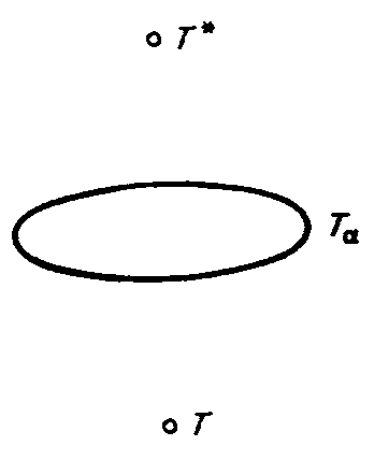
\includegraphics[width = 3 cm]{spectrumTalpha.png}
    \caption{The self-adjoint extensions of $\op T$.}
\end{figure}

\end{example}

\setcounter{section}{6}

\section{Spectral Theorem}

\subsection{The continuous functional calculus}

In this chapter, we will discuss the spectral theorem in its many guises. This structure theorem is a concrete description of all self-adjoint operators. There are several apparently distinct formulations of the spectral theorem. In some sense they are all equivalent.

The form we prefer says that every bounded self-adjoint operator is a multiplication operator. (We emphasize the word bounded since we will deal extensively with unbounded self-adjoint operators in the next chapter; there is a spectral theorem for unbounded operators which we discuss in Section VIII.3.) This means that given a bounded self-adjoint operator on a Hilbert space $\H$, we can always find a measure $\mu$ on a measure space $M$ and a unitary operator $\op U: \H \to \L{2}{M, \D \mu}$ so that
\begin{align}
    (\op U \op A \op U^{-1} f)(x) = F(x)f(x)
\end{align}
for some bounded real-valued measurable function $F$ on $M$.

This is clearly a generalization of the finite-dimensional theorem, which says any self-adjoint $n \times n$ matrix can be diagonalized, or in an abstract form: Given self-adjoint operator $\op A$ on an $n$-dimensional complex space $V$,
there is a unitary operator $\op U: V \to \C^n$ and real numbers $\lambda_1, \cdots, \lambda_n$ so that \begin{align}
    (\op U \op A \op U^{-1} f)_i = \lambda_i f_i \quad \text{for each} \quad f = (f_1, \cdots, f_n) \in \C^n \:.
\end{align}

In practice, $M$ will be a union of copies of $\R$ and $F$ will be $x$, so the core of the proof of the theorem will be the construction of certain measures.
This will be done in Section VII.2 by using the Riesz-Markov theorem.
\footnote{
    The Riesz-Markov theorem reads as follows: Let $X$ be a compact Hausdorff space. For any positive linear functional $\ell$ on $C(X)$ there is a unique Baire measure $\mu$ on $X$ with 
\begin{align*} 
    \ell(f) = \int_X f \, \D \mu \quad \text{for every} \quad f \in C(X) \:.
\end{align*}
}
 Our goal in this section will be to make sense out of $f(\op A)$, for $f$ a continuous function. In the next section, we will consider the measures defined by the functionals $f \mapsto [\psi, f(\op A) \psi]$ for fixed $\psi \in \H$.

Given a fixed operator $\op A$, for which $f$ can define $f(\op A)$?
First, suppose that $\op A$ is an arbitrary bounded operator. If $f(x) = \sum_{n=1}^N a_n x^n$ is a polynomial, we want $f(\op A) = \sum_{n=1}^N a_n \op A^n$. Suppose that $f(x) = \sum_{n=0}^\infty c_n x^n$ is a power series with radius of convergence $R$. If $\norm{A} \leq R$, then $\sum_{n=0}^\infty c_n \op A^n$ converges in $\mathcal{L}(\H)$ so it is natural to set $f(A) = \sum_{n=0}^\infty c_n \op A^n$. In this last case, $f$ was a function analytic in a domain including all of $\sigma(\op A)$. In general, one can make a reasonable definition for $f(\op A)$ if $f$ is analytic in a neighborhood of $\sigma(\op A)$ (see the Notes).

The functional calculus we have talked about thus far works for any operator in any Banach space. The special property of self-adjoint operators (or more generally normal operators; see Problems 3, 5) is that $\norm{P(\op A)} = \sup_{\lambda \in \sigma (\op A)} |P(\lambda)|$ for any polynomial $P$, so that one can use the B.L.T. theorem to extend the functional calculus to continuous functions. Our major goal in this section is the proof of:

\begin{theorem}[Continuous functional calculus] \label{Theorem VII.1}
    Let $\op A$ be a self-adjoint operator on a Hilbert space $\H$. Then there is a \textit{unique} map $\phimap: C(\sigma(\op A)) \to \mathcal{L}(\H)$ with the following properties:
    \begin{enumerate}
        \item $\phimap$ is an algebraic $\star$-homomorphism, that is,
        \begin{align}
            \phimap(fg) = \phimap(f) \phimap(g) \:, \quad \phimap(\lambda f) = \lambda \phimap(f) \:, \\
            \phimap(1) = \op I \:, \quad \phimap(\o{f}) = \phimap(f)^\star \:. 
        \end{align}
        \item $\phi$ is continuous, that is, $\norm{\phi(f)}_{\mathcal{L}(\H)} \leq C \norm{f}_{\infty}$.
        \item Let $f$ be the function $f(x) = x$; then $\phimap(f) = \op A$.
        
        Moreover, $\phimap$ has the additional properties:

        \item If $\op A \psi = \lambda \psi$, then $\phimap(f) \psi = f(\lambda) \psi$.
        \item $\sigma[\phimap(f)] = \set{f(\lambda) | \lambda \in \sigma(\op A)}$ (spectral mapping theorem).
        \item If $f \geq 0$, then $\phimap(f) \geq 0$.
        \item $\norm{\phimap(f)} = \norm{f}_{\infty}$ (this strengthens (2)). 
    \end{enumerate}
\end{theorem}

We sometimes write $\phimap_A(f)$ or $f(\op A)$ for $\phimap(f)$ to emphasize the dependence on $\op A$.

The idea of the proof which we give below is quite simple. (1) and (3) uniquely determine $\phimap(\op P)$ for any polynomial $P(x)$. By the Weierstrass theorem, the set of polynomials is dense in $C(\sigma( \op A))$ so the heart of the proof is showing that
\begin{align}
    \norm{P(\op A)}_{\mathcal{L}(\H)} = \norm{P(x)}_{C(\sigma(\op A)) } = \sup_{\lambda \in \sigma(\op A)} |P(\lambda)| \:.
\end{align}
The existence and uniqueness of $\phimap$ then follow from the B.L.T. theorem.
To prove the crucial equality, we first prove a special case of (5) (which holds for arbitrary bounded operators):

\begin{lemma} \label{Lemma VII.1}
    Let $P(x) = \sum_{n=0}^N a_n x^n$. Let $P(\op A) = \sum_{n=0}^N a_n \op A^n$. Then \begin{align}
        \sigma(P(\op A)) = \set{P(\lambda) | \lambda \in \sigma(\op A)} \:.
    \end{align}
\end{lemma}

\begin{proof}
    Let $\lambda \in \sigma(\op A)$. Since $x = \lambda$ is a root of $P(x) - P(\lambda)$, we have $P(x)- P(\lambda) = (x-\lambda) Q(x)$, so $P(\op A) - P(\lambda) = (\op A - \lambda) Q(\op A)$.
    Since $(\op A - \lambda)$ has no inverse neither does $P(\op A) - P(\lambda)$, that is, $P(\lambda) \in \sigma(P(\op A))$.

    Conversely, let $\mu \in \sigma(P(\op A))$ and let $\lambda_1, \cdots, \lambda_n$ be the roots of $P(x)- \mu$, that is, $P(x) - \mu = a (x-\lambda_1) \cdots (x- \lambda_n)$. If $\lambda_1, \cdots, \lambda_n \notin \sigma(\op A)$, then \begin{align}
        \left[ P(\op A) - \mu \right]^{-1} = a^{-1} (\op A - \lambda_1)^{-1} \cdots (\op A - \lambda_n)^{-1}
    \end{align}
    so we conclude that some $\lambda_i \in \sigma(\op A)$, that is, $\mu = P(\lambda)$ for some $\lambda \in \sigma(\op A)$.
\end{proof}

\begin{lemma}
    Let $\op A$ be a bounded self-adjoint operator. Then
    \begin{align}
        \norm{P(\op A)} = \sup_{\lambda \in \sigma (\op A)} |P(\lambda)| \:.
    \end{align}
\end{lemma}

\begin{proof}
    \begin{align}
        \norm{P(\op A)}^2 =& \norm{P(\op A)^\star P(\op A)} = \norm{(\o{P} P)(\op A)} 
        = \\
        =& \sup_{\lambda \in \sigma [(\o{P} P)(\op A)]} |\lambda| \quad \text{(by Theorem VI.6)} \nonumber \\
        =& \sup_{\lambda \in \sigma(\op A)} |(\o{P} P)(\lambda)| \quad \text{(by Lemma \ref{Lemma VII.1})}  \nonumber \\
        =& \left( \sup_{\lambda \in \sigma(\op A)} |P(\lambda)| \right)^2 \:. \nonumber
    \end{align}
\end{proof}

\begin{proof}[Proof of Theorem \ref{Theorem VII.1}]
    Let $\phimap(P) = P(\op A)$. Then $ \norm{\phimap(P)}_{\mathcal L(\H)} = \norm{P}_{C(\sigma(\op A))} $, so $\phimap$ has a unique linear extension to the closure of the polynomials in $C(\sigma(\op A))$. Since the polynomials are an algebra containing $1$, containing complex conjugates, and separating points, this closure is all of $C(\sigma(\op A))$. 
    
    Properties (1), (2), (3), (7) are obvious and if $\hat \phimap$ obeys (1), (2), (3) it agrees with $\phimap$ on polynomials and thus by continuity on $C(\sigma(\op A))$. 
    
    To prove (4), note that $\phimap(P)\psi = P(\lambda) \psi$ and apply continuity. 
    
    To prove (6), notice that if $f \geq 0$, then $f = g^2$ with $g$ real and $g \in C(\sigma( \op A))$. Thus $\phimap(f) = \phimap(g)^2$ with $\phimap(g)$ self-adjoint, so $\phimap(f) \geq 0$.

    Finally, (5) is left for the reader (Problem 8).
    
\end{proof}

Before turning to some examples, we make several remarks:
\begin{enumerate}
    \item $\phimap(f) \geq 0$ if and only if $f \geq 0$ (Problem 9).
    
    \item Since $fg = gf$ for all $f$ and $g$, the set $\set{f(\op A) | f \in C(\sigma(\op A))}$ forms an abelian algebra closed under adjoints. Since $\norm{f(\op A)} = \norm{f}_\infty$ and $C(\sigma( \op A))$ is complete, $\set{f(\op A) | f \in C(\sigma(\op A))}$ is norm-closed. It is thus an \textbf{abelian $C^\star$ algebra} of operators. 
    \item $\Ran (\phimap)$ is actually the $C^\star$ \textbf{algebra generated by} $\op A$, that is, the smallest $C^\star$-algebra containing $\op A$ (Problem 10).
    \item This result, that $C(\sigma (\op A))$ and the $C^\star$-algebra generated by $\op A$ are isometrically isomorphic, is actually a special case of the \enquote{commutative Gelfand-Naimark theorem} which we discuss in Chapter XV.
    \item The statement (2) actually follows from (1) and abstract nonsense (Problem 11). Thus (1) and (3) alone determine $\phimap$ uniquely.
    
\end{enumerate}

Finally, we consider two specific examples of $\phimap(f)$:

\begin{example}
    As a corollary, we have a new proof of the existence half of the square-root lemma (Theorem VI.9) for if $\op A \geq 0$, then $\sigma (\op A) \subset  [0, \infty)$ (Problem 12). If $f(x) = x^{1/2}$, then $f(\op A)^2 = \op A$.
\end{example}

\begin{example}
    From (7) of Theorem \ref{Theorem VII.1}, we see that $\norm{(\op A - \lambda)^{-1}} = \left[ \mathrm{dist}\, (\lambda, \sigma(\op A)) \right]^{-1}$ if $\op A$ is bounded, self-adjoint, and $\lambda \notin \sigma(\op A)$.
\end{example}

\subsection{The spectral measures}

We are now ready to introduce the measures we have anticipated so often before. Let us fix $\op A$, a bounded self-adjoint operator. Let $\psi \in \H$. 
Then $f \mapsto (\psi, f(\op A) \psi)$ is a positive linear functional on $C(\sigma(\op A))$. Thus, by the Riesz-Markov theorem (Theorem IV.14), there is a unique measure $\mu_\psi$ on the compact set $\sigma(\op A)$ with 
\begin{align}
    (\psi, f(\op A) \psi) = \int_{\sigma (\op A)} f(\lambda) \, \D \mu_\psi \:.
\end{align}

\begin{definition}
    The measure $\mu_\psi$ is called the \textbf{spectral measure associated with the vector} $\psi$.
\end{definition}

The first and simplest application of the $\mu_\psi$ is to allow us to extend the functional calculus to $\mathcal B(\R)$, the bounded Borel functions on $\R$. Let $g \in \mathcal B(\R)$. It is natural to define $g(\op A)$ so that 
\begin{align}
    (\psi, g(\op A) \psi) = \int_{\sigma (\op A)} g(\lambda) \, \D \mu_\psi (\lambda) \:.
\end{align}
The polarization identity lets us recover $(\psi, g(\op A) \phi)$ from the proposed $(\psi, g(\op A) \psi)$ and then the Riesz lemma lets us construct $g(\op A)$. The properties of this \enquote{measurable functional calculus} are given in (Problem 13):

\footnote{The polarization identity: \begin{align*}
    4 (x,y) = \left(\norm{x+y}^2 - \norm{x-y}^2 \right) - i \left(\norm{x+iy}^2 - i \norm{x - iy}^2 \right) \:.
\end{align*} }

\begin{theorem}[Spectral theorem - functional calculus form]
    Let $\op A$ be a bounded self-adjoint operator in $\H$. There is a unique map $\hat \phimap: \mathcal B(\R) \to \mathcal L (\H)$ so that \begin{enumerate}
        \item $\hat \phimap$ is an algebraic $\star$-homomorphism.
        \item $\hat \phimap$ is norm continuous: $\norm{\hat \phimap (f)}_{\mathcal L(\H)} = \norm{f}_\infty$.
        \item Let $f$ be the function $f(x) = x $; then $\hat \phimap(f) = \op A$.
        \item Suppose $f_n(x) \rightarrow f(x)$ for each $x$ and $\norm{f_n}_\infty$ is bounded. Then $\hat \phimap(f_n) \rightarrow \hat \phimap (f)$ strongly.
    \end{enumerate}
    
    Moreover, $\hat \phimap$ has the properties:
    \begin{enumerate}
        \item If\, $\op A \psi = \lambda \psi$, the $\hat \phimap(f) \psi = f(\lambda) \psi$.
        \item If\, $f \geq 0$, then $\hat \phimap (f) \geq 0$.
        \item If\, $\op B \op A = \op A \op B$, then $\hat \phimap (f) \op B = \op B \hat \phimap(f)$.
    \end{enumerate}
\end{theorem}

Theorem VII.2 can be proven directly by extending Theorem VII.1; part (4) requires the dominated convergence theorem. Or, Theorem VII.2 can be proven by an easy corollary of Theorem VII.3 below. The proof of Theorem VIL3 uses only the \textit{continuous} functional calculus. $\hat \phimap$ extends $\phimap$ and as before we write $\hat \phimap (f) = f(\op A)$. As in the continuous functional calculus, one has $f(\op A) g(\op A) = g(\op A) f(\op A)$.
Since $\mathcal B (\R)$ is the smallest family closed under limits of form (4) containing all of $C(\R)$, we know that any $\hat \phimap$ is in the smallest $C^\star$-algebra containing $\op A$ which is also strongly closed; such an algebra is called a von Neumann or $W^\star$-algebra. When we study von Neumann algebras in Chapter XVIII we will see that this follows from (7).
The norm equality of Theorem VII.I carries over if we define $\norm{f}_\infty '$, to be the $L^\infty$-norm with respect to a suitable notion of \enquote{almost everywhere}. Namely, pick an orthonormal basis $\set{\psi_n}$ and say that a property is true a.e. if it is true a.e. with respect to \textit{each} $\mu_{\psi_i}$. Then $\norm{ \hat \phimap (f)}_{\mathcal L(\H)} =\norm{f}_\infty '$.
In the next section, we will return to the operators $\chi_\Omega (\op A)$ where $\chi_\Omega$ is a characteristic function; this is the most important set of operators in the measurable but not in the continuous functional calculus. For the time being, we turn to using the spectral measures to form $L^2$ spaces. We first define:

\begin{definition}
    A vector $\psi \in \H$ is called a \textbf{cyclic vector} for $\op A$ if finite linear combinations of the elements $\set{\op A^n \psi}_{n=0}^\infty$ are dense in $\H$.
\end{definition}

Not all operators have cyclic vectors (Problem 14), but if they do:

\begin{lemma}
    Let $\op A$ be a bounded self-adjoint operator with cyclic vector $\psi$. Then, there is a unitary operator $\op U: \H \to \L{2}{\sigma(\op A), \D \mu_\psi}$ with \begin{align}
        (\op U \op A \op U^{-1} f) (\lambda) = \lambda f(\lambda) \:.
    \end{align}
    Equality is in the sense of elements of $\L{2}{\sigma(\op A), \D \mu_\psi}$.
\end{lemma}

\begin{proof}
    Define $\op U$ by $\op U \phimap(f) \psi \equiv f$ where $f$ is continuous. $\op U$ is essentially the inverse of the map $\phimap$ of Theorem \ref{Theorem VII.1}. To show that $\op U$ is well defined we compute
    \begin{align}
        \norm{\phimap(f) \psi}^2 = \left( \psi, \phimap^\star (f) \phimap(f) \psi \right) = \left( \psi, \phimap (\o f f) \psi \right) = \int |f(\lambda)|^2 \, \D \mu_\psi \:.
    \end{align}
    Therefore, if $f=g$ a.e. with respect to $\mu_\psi$, then $\phimap(f) \psi = \phimap(g) \psi$. Thus $\op U$ is well defined on $\set{\phimap(f) | f \in C (\sigma (\op A))}$ and is norm preserving. Since $\psi$ is cyclic, \begin{align}
        \o{ \set{ \phimap(f) \psi | f \in C (\sigma (\op A))  } } = \H \:,
    \end{align}
    so by the B.L.T. theorem $\op U$ extends to an isometric map of $\H$ into $\L{2}{\sigma(\op A), \D \mu_\psi}$. Since $C(\sigma (\op A))$ is dense in $L^2$, $\Ran \op U = \L{2}{\sigma(\op A), \D \mu_\psi}$. Finally, if $f \in C(\sigma (\op A))$, \begin{align}
        (\op U \op A \op U^{-1} f )(\lambda) = [\op U \op A \phimap(f)](\lambda) = [\op U \phimap(xf)](\lambda) = \lambda f (\lambda) \:.
    \end{align}
    By continuity, this extends from $f \in C(\sigma (\op A))$ to $f \in L^2$.
\end{proof}

To extend this lemma to arbitrary $\op A$, we need to know that $\op A$ has a family of invariant subspaces spanning $\H$ so that $\op A$ is cyclic on each subspace:

\begin{lemma}
    Let $\op A$ be a self-adjoint operator on a separable Hilbert space $\H$. Then there is a direct sum decomposition $\H = \oplus_{n=1}^N \H_n$ with $N=1,2, \cdots $ or $\infty$ so that:
    \begin{enumerate}
        \item $\op A$ leaves each $\H_n$ \textbf{invariant}, that is, $\psi \in \H_n$ implies $\op A \psi \in \H_n$.
        \item For each $n$, there is a $\phi_n \in \H_n$ which is cyclic for $\op A |_{\H_n}$, i.e.
        \begin{align}
            \H_n = \o{ \set{ f(\op A) \phi_n | f \in C(\sigma (\op A)) } } \:.
        \end{align}
    \end{enumerate} 
\end{lemma}

\begin{proof}
    A simple Zornication\footnote{Don't know what that means\dots} (Problem 15).
\end{proof}

We can now combine Lemmas 1 and 2 to prove the form of the spectral theorem which we regard as the most transparent:

\begin{theorem}[Spectral theorem - multiplication operator form]
    Let $\op A$ be a bounded self-adjoint operator on $\H$, a separable Hilbert space. Then, there exist measures $\set{\mu_n}_{n=1}^N$, ($N = 1,2,\cdots$ or $\infty$) on $\sigma(\op A)$ and a unitary operator
    \begin{align}
        \op U : \H \to \bigoplus_{n=1}^N \L{2}{\R, \D \mu_n}
    \end{align}
    so that \begin{align}
        (\op U \op A \op U^{-1} \psi)_n (\lambda) = \lambda \psi_n(\lambda) \:,
    \end{align}
    where we wrie an element $\psi \in \oplus_{n=1}^N \L{2}{\R, \D \mu_n}$ as an $N$-tuple $[\psi_1(\lambda), \cdots, \psi_N(\lambda)]$. This realization of $\op A$ is called a \textbf{spectral representation}.
\end{theorem}

\begin{proof}
    Use Lemma 2 to find the decomposition and then use Lemma 1 on each component.
\end{proof}

This theorem tells us that every bounded self-adjoint operator is a multiplication operator on a suitable measure space; what changes as the operator changes are the underlying measures. Explicitly:

\begin{corollary}
    Let $\op A$ be a bounded self-adjoint operator on a separable Hilbert space $\H$. Then there exists a finite measure space $(M, \mu)$ a bounded function $F$ on $M$, and a unitary map, $ \op U: \H \to \L{2}{M, \D \mu}$, so that
    \begin{align}
        (\op U \op A \op U^{-1} f) (m) = F(m) f(m) \:.
    \end{align}
\end{corollary}

\begin{proof}
    Choose the cyclic vectors $\phi_n$, so that $\norm{\phi_n} = 2^{-n}$. Let $M = \cup_{n=1}^N \R$ i.e. the union of $N$ copies of $\R$. Define $\mu$ by requiring that its restriction to the nth copy of $\R$ be $\mu_n$. Since $\mu(M) = \sum_{n=1}^N \mu_n(\R) < \infty$, $\mu$ is finite.
\end{proof}

We also notice that this last theorem is essentially a rigorous form of the physicist's Dirac notation.
If we write $\psi_n(x) = \psi(x;n)$, we see that in the \enquote{new representation defined by U} one has
\begin{align}
    (\psi, \phi) =& \sum_n \int \, \D \mu_n \o{ \psi(\lambda; n)} \phi(\lambda; n) \:, \\
    (\psi, \op A \phi) =& \sum_n \int \, \D \mu_n \o{ \psi(\lambda; n)} \lambda \phi(\lambda; n) \:.
\end{align}

These are the Dirac type formulas familiar to physicists except that the formal sums of Dirac are replaced with integrals over spectral measures, where we define:

\begin{definition}
    The measures $\D \mu_n$ are called \textbf{spectral measures}; they are just $\D \mu_\psi$ for suitable $\psi$.
\end{definition}

These measures are not uniquely determined and we will eventually discuss this nonuniqueness question. First, let us consider a few examples:

\begin{example}
Let $\op A$ be an $n \times n$ self-adjoint matrix. The \enquote{usual} finite- dimensional spectral theorem says that $\op A$ has a complete orthonormal set of eigenvectors, $\psi_1, \cdots, \psi_n$ with $\op A \psi_i = \lambda_i \psi_i$. Suppose first that the eigenvalues are distinct.
Consider the sum of Dirac measures, $\mu = \sum_{i=1}^n a_i \delta(x-\lambda_i)$. $\L{2}{\R, \D \mu} $ is just $\C^n$ since $f \in L^2$ is determined by $f = [f(\lambda_1), \cdots, f(\lambda_n)]$.
Clearly, the function $\lambda f$ corresponds to the $n$-tuple $f = [\lambda_1 f(\lambda_1), \cdots, \lambda_n f(\lambda_n)]$ so $\op A$ is multiplication by $\lambda$ on $\L{2}{\R, \D \mu}$. If we take $\tilde \mu = \sum_{i=1}^n a_o \delta(x-\lambda_i)$ with $a_1, \dots, a_n >0$, $\op A$ can also be represented as multiplication by $\lambda$ on $\L{2}{\R, \D \tilde \mu}$. Thus, we explicitly see the nonuniqueness of the measure in this case. We can also see when more than one measure is needed: one can represent a finite-dimensional self-adjoint operator as multiplication on $\L{2}{\R, \D \tilde \mu}$ with only one measure if and only if $\op A$ has no repeated eigenvalues.
\end{example}

\begin{example}
Let $\op A$ be compact and self-adjoint. The Hilbert-Schmidt theorem tells us there is a complete orthonormal set of eigenvectors $\set{\psi_n}_{n=1}^\infty$ with $\op A \psi_n = \lambda_n \psi_n$. If there is no repeated eigenvalue, $\sum_{n=1}^\infty 2^{-n} \delta(x-\lambda_n)$ works as a spectral measure.
\end{example}

\begin{example}
Let $\H = l^2(-\infty, +\infty)$, that is, the set of sequences, $\set{a_n}_{n=-\infty}^{+\infty}$ with $\sum_{n=-\infty}^{+\infty} |a_n|^2 < \infty$. Let $\op L : \H \to \H$ by $(\op L a)_n = a_{n+1}$, that is, $\op L$ shifts to the left. $\op L^\star = \op R$ with $(\op R a)_n = a_{n-1}$. Let $\op A = \op R + \op L$ which is self-adjoint. Can we represent $\op A$ as a multiplication operator? Map $\H$ into $\L{2}{[0,1]}$ by $\op U: \set{a_n} \mapsto \sum_{n=-\infty}^\infty a_n e^{2 \pi i n x}$.
Then $\op U \op L \op U^{-1}$ is multiplication by $e^{-2 \pi i x}$ and $\op U \op R \op U^{-1}$ is multiplication by $e^{+2 \pi i x}$ so $\op U \op A \op U^{-1}$ is multiplication by $2 cos( 2 \pi x)$. 
The necessary transformations needed to represent $\op A$ as multiplication by $x$ on $\L{2}{\R, \D \mu_1} \oplus \L{2}{\R, \D \mu_2} $ are left for the problems. $\mu_1$ and $\mu_2$ have support in $[-2, 2]$.
\end{example}

\begin{example}
Consider $\frac{1}{i} \der{}{x}$ on $\L{2}{\R, \D x}$. This is an unbounded operator and thus not strictly within the context of this section, but we will prove an analogue of Theorem VII.3 in Section VIII3. We thus seek an operator $\op U$ and a measure $\D \mu$ (it turns out that only one $\mu$ is needed) with $\op U : \L{2}{\R, \D x} \to \L{2}{\R, \D \mu(k)}$ so that
\begin{align}
    \op U \left( \frac{1}{i} \der{f}{x} \right) (k) = k \op U f(k) \:.
\end{align}
The Fourier transform $(\op U f)(k) = \frac{1}{\sqrt{2 \pi}} \int f(x) e^{-ikx} \, \D x$ which we study in Chapter IX precisely does the trick. Thus, the Fourier transform is one example of a spectral representation.
\end{example}

We now investigate the connection between spectral measures and the
spectrum.

\begin{definition}
    If $\set{\mu_n}_{n=1}^N$ is a family of measures, the \textbf{support} of $\set{\mu_n}$ is the complement of the largest open set $B$ with $\mu_n (B) = 0$ for all $n$; so \begin{align}
        \supp \set{\mu_n} = \o { \bigcup_{n=1}^N \supp \mu_n } \:.
    \end{align}
\end{definition}

\begin{proposition}
    Let $\op A$ be a self-adjoint operator and $\set{\mu_n}_{n=1}^N$ a family of spectal measures. Then \begin{align}
        \sigma(\op A) = \supp \set{\mu_n}_{n=1}^N \:.
    \end{align}
\end{proposition}

There is also a simple description of $\sigma(\op A)$ in terms of the more multiplication operators discussed after Theorem VII.3:

\begin{definition}
    Let $F$ be a real-valued function on a measure space $(M, \mu)$. We say $\lambda$ is in the \textbf{essential range} of $F$ if and only if \begin{align}
        \forall \varepsilon > 0 \: : \quad  \mu \set{m | \lambda - \varepsilon < F(m) < \lambda + \varepsilon } > 0 \:.
    \end{align}
\end{definition}

\begin{proposition}
    Let $F$ be a real-valued function on a measure space $(M, \mu)$. Let $\op T_F$ be the operator on $\L{2}{M, \D \mu}$ given by \begin{align}
        (\op T_F g)(m) = F(m) g(m) \:.
    \end{align}
    Then $\sigma(\op T_F)$ is the essential range of $F$.
\end{proposition}

\begin{proof}
    See Problem 17b.
\end{proof}

We can now see exactly what information is contained in the spectrum. A unitary invariant of a self-adjoint operator $\op A$ is a property $P$ so that $P(\op A) = P(\op U \op A \op U^{-1})$ for all unitary operators $\op U$. Thus, unitary invariants are \enquote{intrinsic} properties of self-adjoint operators, that is, properties independent of \enquote{representation}. An example of such a unitary invariant is the spectrum $\sigma( \op A)$. However, the spectrum is a poor invariant: for example, multiplication by $x$ on $\L{2}{[0,1], \D x}$ and an operator with a complete set of eigenfunctions having all rationals in $[0, 1]$ as eigenvalues are very different even though both have spectrum $[0, 1]$.
At the conclusion of this section, we will see that there is a canonical choice of “spectral measures” which forms a complete set of unitary invariants, that is, a set of properties which distinguish two self-adjoint operators $\op A$ and $\op B$ unless $\op A = \op U \op B \op U^{-1} $ for some unitary operator $\op U$. This explains why $\sigma (\op A)$ is such a bad invariant for different sorts of measures can have the same support. If we wish to find better invariants which are, however, simpler than measures, it is reasonable to first decompose spectral measures in some natural way and then pass to supports.
Recall Theorem I.13 which says that any measure $\mu$ on $\R$ has a unique decomposition into $\mu = \mupp + \muac + \musing $ where $\mupp$ is a pure point measure, $\muac$ is absolutely continuous with respect to Lebesgue measure, and $\musing$ is continuous and singular with respect to Lebesgue measure. These three pieces are mutually singular so
\begin{align}
    \L{2}{\R, \D \mu} = \L{2}{\R, \D \mupp} \oplus \L{2}{\R, \D \muac} \oplus \L{2}{\R, \D \musing} \:.
\end{align}
It is easy to see (Problem 18) that any $\psi \in \L{2}{\R, \D \mu}$ has an absolutely continuous spectral measure $\D \mu_\psi$ if and only if $\psi \in \L{2}{\R, \D \mu}$ and similarly for pure point and singular measures. If $\set{\mu_n}_{n=1}^N$ is a family of spectral measures, we can sum $\oplus_{n=1}^N \L{2}{\D \mu_{n ; \mathrm{ac}}}$ by defining:

\begin{definition}
    Let $\op A$ be a bounded self-adjoint operator on $\H$. Let $\Hpp = \set{\psi | \mu_\psi \text{ is pure point}}$, $\Hac = \set{\psi | \mu_\psi \text{ is absolutely continuous}}$ and $ \Hsing = \set{\psi | \mu_\psi \text{ is continuous singular}}$.
\end{definition}

We have thus proven:

\begin{theorem}
    $\H = \Hpp \oplus \Hac \oplus \Hsing$. Each of these subspaces is invariant under $\op A$. $\op A|_{\Hpp}$ is a complete set of eigenvectors, $\op A|_{\Hac}$ has only absolutely continuous spectral measures and $\op A|_{\Hsing}$ has only continuous singular spectral measures.
\end{theorem}

%%-------------------------------------
%	BIBLIOGRAPHY
%-------------------------------------

\renewcommand{\refname}{\spacedlowsmallcaps{References}} % For modifying the bibliography heading

\bibliographystyle{unsrt}

\bibliography{sample.bib} % The file containing the bibliography

%------------------------------------

\end{document}
